\graphicspath{{appendix/images/}}

\begin{frame}
	\begin{center}
		\begin{Large}
			Andrei Yauseyenka
		\end{Large}
	\end{center}
\end{frame}

\begin{frame}{Anforderung}
	\begin{itemize}
		\item Übergabe der Daten an die Unity Gruppe
		\item Übergabe der Daten an die CityGML Gruppe
		\item Teilszenarien auslesen können
		\item Mithilfe an den Modell für das Pferd
	\end{itemize}
\end{frame}

\begin{frame}{Meine Aufgaben}
	\begin{itemize}
		\item Scrum Master
		\item Output Dateien Konfigurieren(Zusammen mit Daniel)
		\item Output für CityGML (Vorarbeit erhalten von Florian)
		\item Szenario Landshut
		\begin{itemize}
			\item Szenario von der CityGML Gruppe einlesen (Erhalten von Lesya)
			\item Topography Performance (Zusammen mit Nikolai)
		\end{itemize}
		\item Test Klassen geschrieben für VEllipse
		\item Modellattribute festlegen und implementieren
	\end{itemize}
\end{frame}

\begin{frame}{Scrum Master}
	\begin{itemize}
		\item Sprintplannung 
		\item Aufgabenverteilung an die Teammitglieder
		\item Projektübersicht
		\item Leitung der Daylies
		\item Kontaktperson für die anderen Gruppen.
	\end{itemize}
\end{frame}

\begin{frame}{Modellattribute}
Einführung von verschiedenen Eigenschaften die ein Pferd besitzen kann.
\begin{itemize}
	\item Scheuklappen\cite{Wikipedia-Scheuklappen}
	\begin{itemize}
		\item Sehwinkel eines Pferdes ohne Scheuklappe: 270\degree \cite{barnboox.de}
		\item Sichtfeld des Pferdes wird beeinträchtigt
		\item Folge: Einschränkung des Drehwinkels
	\end{itemize}
	\item Reiter
	\begin{itemize}
		\item Pferd wiegt schwerer
		\item Folge: Die Geschwindigkeit des Pferdes wird verlangsamt
	\end{itemize}
\end{itemize}
\end{frame}

\begin{frame}{Landshut Teil Szenario}
	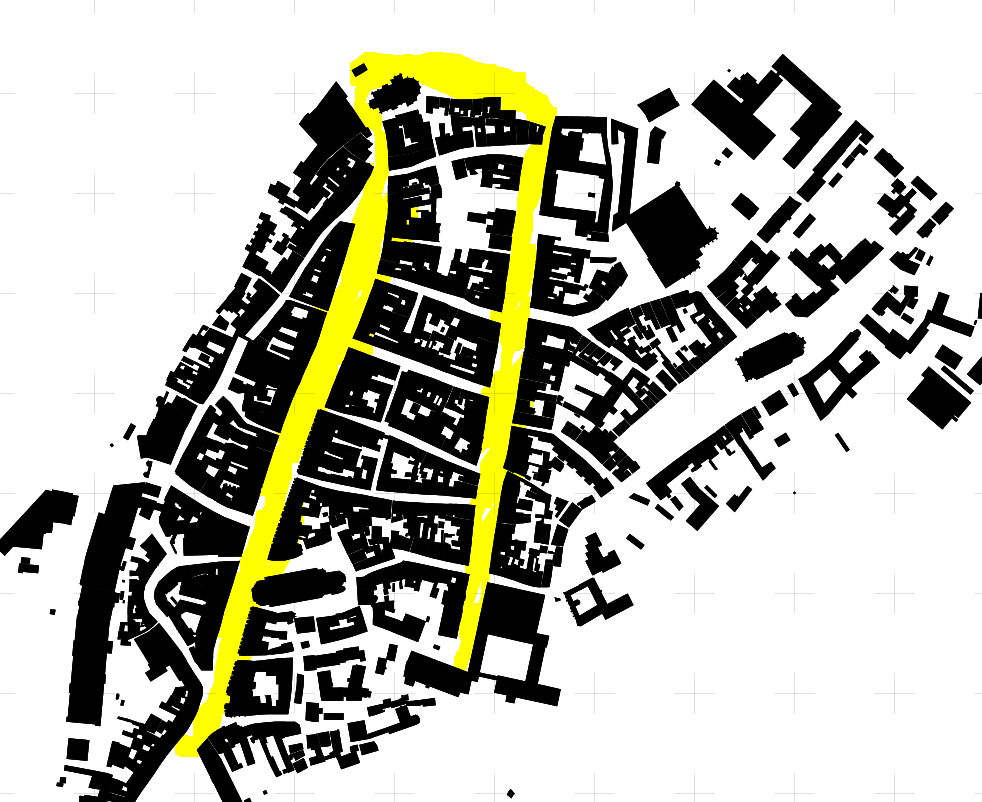
\includegraphics[width=\textwidth]{./LandshutRoute.png}
\end{frame}

\begin{frame}{Landshut Teil Szenario}
	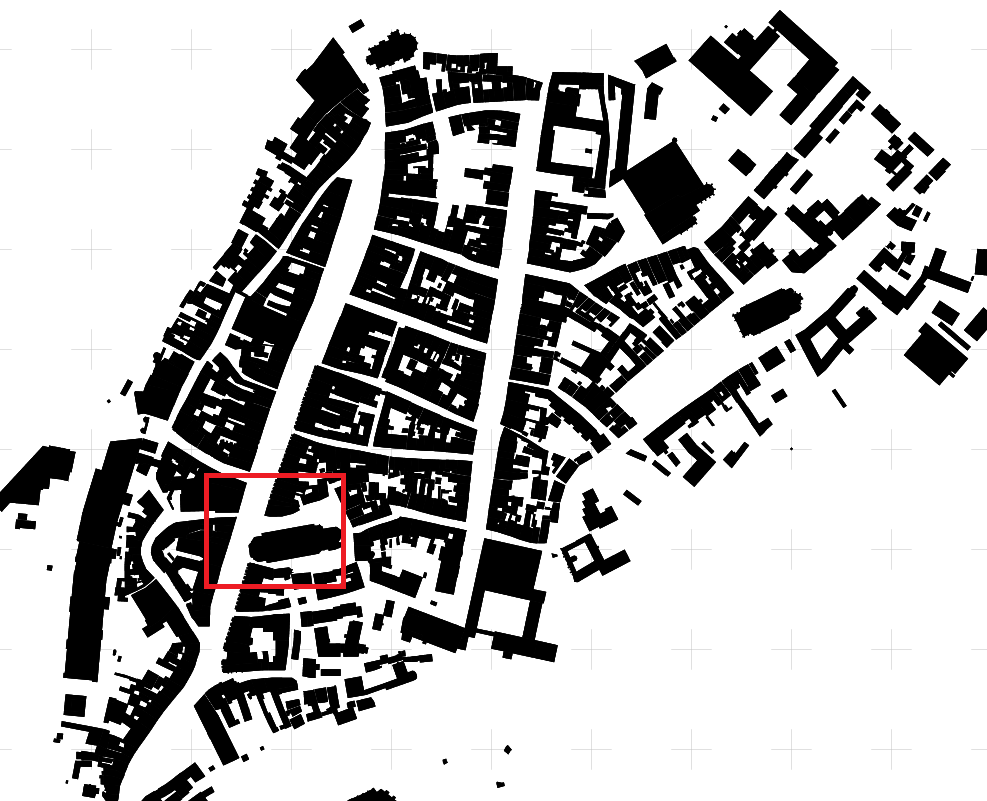
\includegraphics[width=\textwidth]{./LandshutFull.png}
\end{frame}

\begin{frame}{Landshut Teil Szenario}
	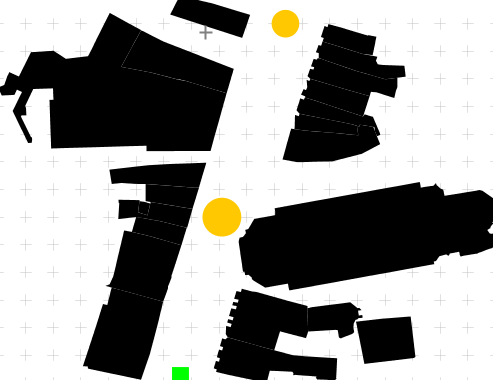
\includegraphics[width=\textwidth]{./LandshutTeilausschnitt.png}
\end{frame}

\begin{frame}{Landshut Teil Szenario}
	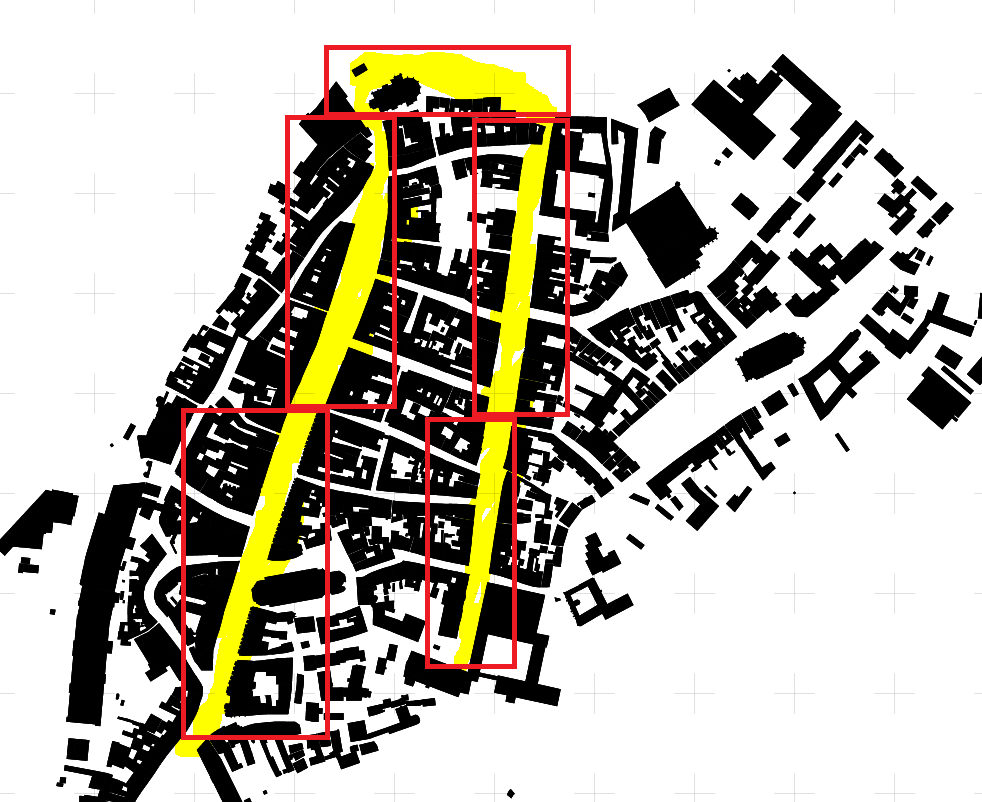
\includegraphics[width=\textwidth]{./LandshutRouteTeile.png}
\end{frame}

\begin{frame}{Fazit}
	\begin{itemize}
		\item Unity Gruppe bekommt Daten
		\item Erfolgreiches abspielen eines Szenarios
		\item Modell wurde erweitert
		\item Prozessoren müssen noch optimiert werden für die CityGML Gruppe
	\end{itemize}
\end{frame}

\begin{frame}{Retrospektive}
	\begin{itemize}
		\item{Fand ich gut:}
		\begin{itemize}
			\item{Hilfebereitschaft des Teams}
		\end{itemize}
		\item{Könnte besser sein:}
		\begin{itemize}
			\item{Tasks sollten nur in der Daily erstellt werden}
		\end{itemize}
		\item{Mein Anteil: 23\%}
	\end{itemize}
\end{frame}